%!TEX TS-program = pdflatex
\documentclass[a4paper,12pt,twoside]{article}

\usepackage{mathptmx}
\usepackage{parskip}
\usepackage[top=1.5in,left=1in,right=1in,bottom=1in]{geometry}
%\setlength{\parindent}{0pt}
%\setlength{\parskip}{\the\baselineskip}
\pagestyle{empty} 

\makeatletter
\renewcommand\@makefntext[1]{%
  \parindent 1em\noindent
  \hbox{\@makefnmark}#1}
\renewcommand\large{\@setfontsize\large{14pt}{18}} % For standardizing with the Word template: normally \large is 14.4pt
\makeatother
\usepackage{titlesec}
\titleformat{\subsection}{\normalfont\normalsize}{\thesubsection.}{1ex}{}
\titleformat{\subsubsection}{\normalfont\normalsize}{\thesubsubsection.}{1ex}{}
\titleformat{\section}{\normalfont\normalsize\bfseries}{\thesection.}{1ex}{}
% \titlespacing*{\section}{0pt}{*0}{0pt}
% \titlespacing*{\subsection}{0pt}{\the\baselineskip}{0pt}

\usepackage{natbib} 
\bibpunct{(}{)}{;}{a}{,}{,}


\setlength{\bibsep}{0pt} \relax
\setcitestyle{notesep={: },yysep={, }} \relax

\usepackage{linguex,url}
\def\refdash{} % To suppress the dash in (2-a) etc. Defining both as different versions of linguex had different names for this command.
\def\firstrefdash{}


\usepackage{titleps}
\usepackage{lipsum}
\newpagestyle{mystyle}{
\sethead[\thepage][\Author][]{}{\Title}{\thepage}
}
\pagestyle{mystyle}
\author{Hofmann \and de Marneffe  \and Tonhauser}
\title{Projection variability of clausal complements across different operators}
\makeatletter
\newcommand\Author{Hofmann, de Marneffe, and Tonhauser}
\let\Title\@title
\makeatother
%header with author and title

\pagenumbering{gobble} 
%suppresses page numbering in header


%!TEX root = xprag-poster.tex

%% extra 

% colors

	\definecolor{maintheme}{cmyk}{.71, .51, 0, 0}
	\definecolor{highlight}{cmyk}{.05, .8, .05, 0}
	\definecolor{lowlight}{cmyk}{.64, .5, 0, .09}
	\definecolor{sechighlight}{cmyk}{0, .31, 100, .10}

	% \setbeamercolor{alerted text}{fg=orange}
	\setbeamercolor{background canvas}{bg=white}
	% \setbeamercolor{block body alerted}{bg=normal text.bg!90!black}
	\setbeamercolor{block body}{bg=normal text.bg!90!black}
	% \setbeamercolor{block body example}{bg=normal text.bg!90!black}
	% \setbeamercolor{block title alerted}{use={normal text,alerted text},fg=alerted text.fg!75!normal text.fg,bg=normal text.bg!75!black}
	% \setbeamercolor{block title}{bg=blue}
	% \setbeamercolor{block title example}{use={normal text,example text},fg=example text.fg!75!normal text.fg,bg=normal text.bg!75!black}
	% \setbeamercolor{fine separation line}{}
	% \setbeamercolor{frametitle}{fg=brown}
	% \setbeamercolor{item projected}{fg=black}
	\setbeamercolor{normal text}{fg=black}
	\setbeamercolor{caption name}{fg=black}
	% \setbeamercolor{separation line}{}
	\setbeamercolor{structure}{fg=maintheme}
	\setbeamercolor{title}{fg=maintheme, bg=lowlight}
	% \setbeamercolor{titlelike}{fg=maintheme}

	\definecolor{modal}{cmyk}{0, .31, 100, .0}
	\definecolor{cond}{cmyk}{.8, 0, .3, .3}
	\definecolor{neg}{cmyk}{.63, .23, 0, .0}
	\definecolor{question}{cmyk}{1, .36, 0, .30}

	\definecolor{red}{cmyk}{0,1,.5,0}

% boxes
	\usepackage{tcolorbox}
	\tcbuselibrary{skins}

	\newtcbox{\predhighlight}[1][lowlight]{on line,
	arc=3pt,colback=#1!10!white,colframe=#1!50!black,
	before upper={\rule[-3pt]{0pt}{10pt}},boxrule=1pt,
	boxsep=0pt,left=2pt,right=2pt,top=1pt,bottom=.5pt}

	\newtcbox{\ophighlight}[1][highlight]{on line,
	arc=3pt,colback=#1!10!white,colframe=#1!50!black,
	before upper={\rule[-3pt]{0pt}{10pt}},boxrule=1pt,
	boxsep=0pt,left=2pt,right=2pt,top=1pt,bottom=.5pt}

	\newtcolorbox{normalbox}[1]{colback=white,colframe=maintheme,fonttitle=\bfseries\Raleway\large,
	title={#1}}

	% \tcbset{colback=red!5!white,fonttitle=\bfseries}
	% \newtcolorbox{upshotbox}[1]{enhanced, squeezed title={#1}, frame style={left color=highlight, right color=lowlight!75!black}, leftrule=3mm, fonttitle=\bfseries\Raleway\Large, colback=highlight!5!white
	% }

	\newtcolorbox{upshotbox}[1]{
		colframe=highlight,
		colback=highlight!5!white,
		% colframe=maintheme,
		% colback=white,
		% coltitle=maintheme,
		adjusted title=center,halign title=center,
		title={#1},
		% frame style={left color=highlight, right color=lowlight!75!black},
		leftrule=3mm,
		fonttitle=\bfseries\Raleway\Large,
		%
		% detach title, before upper={\centering\tcbtitle\par}
	}

	\newtcolorbox{modelbox}[1]{
		% colback=lowlight!5!white,
		% colframe=lowlight,
		% coltitle=lowlight,
		colback=white,
		colframe=maintheme,
		coltitle=maintheme,
		text width=.95\linewidth,
		title={#1},
		fonttitle=\bfseries\footnotesize,
		detach title, before upper={\tcbtitle\par},
	}

	\newtcolorbox{theorybox}[1]{
		% colback=lowlight!5!white,
		% coltitle=lowlight,
		% colframe=lowlight,
		colback=white,
		colframe=maintheme,
		coltitle=maintheme,
		text width=.85\linewidth,
		title={#1},
		fonttitle=\bfseries\small,
		detach title, before upper={\tcbtitle\par},
	}

	\newtcolorbox{questionbox}[1]{
		colback=question!5!white,
		colframe=question,
		coltitle=question,
		% text width=.78\linewidth,
		title={#1},
		fonttitle=\bfseries,
		detach title, before upper={\tcbtitle},
	}

	\newtcolorbox{negbox}[1]{
		colback=neg!5!white,
		colframe=neg,
		coltitle=neg,
		% text width=.78\linewidth,
		title={#1},
		fonttitle=\bfseries,
		detach title, before upper={\tcbtitle},
	}

	\newtcolorbox{modalbox}[1]{
		colback=modal!5!white,
		colframe=modal,
		coltitle=modal,
		% text width=.78\linewidth,
		title={#1},
		fonttitle=\bfseries,
		detach title, before upper={\tcbtitle},
	}

	\newtcolorbox{condbox}[1]{
		colback=cond!5!white,
		colframe=cond,
		coltitle=cond,
		% text width=.78\linewidth,
		title={#1},
		fonttitle=\bfseries,
		detach title, before upper={\tcbtitle},
	}

	\newtcbox{\qhl}[1][lowlight]{on line,
	arc=3pt,colback=question!5!white,colframe=question,
	coltitle=question,
	before upper={\rule[-3pt]{0pt}{10pt}},boxrule=1pt,
	boxsep=0pt,left=2pt,right=2pt,top=1pt,bottom=.5pt}

	\newtcbox{\nhl}[1][lowlight]{on line,
	arc=3pt,colback=neg!5!white,colframe=neg,
	coltitle=neg,
	before upper={\rule[-3pt]{0pt}{10pt}},boxrule=1pt,
	boxsep=0pt,left=2pt,right=2pt,top=1pt,bottom=.5pt}

	\newtcbox{\mhl}[1][lowlight]{on line,
	arc=3pt,colback=modal!5!white,colframe=modal,
	coltitle=modal,
	before upper={\rule[-3pt]{0pt}{10pt}},boxrule=1pt,
	boxsep=0pt,left=2pt,right=2pt,top=1pt,bottom=.5pt}

	\newtcbox{\chl}[1][lowlight]{on line,
	arc=3pt,colback=cond!5!white,colframe=cond,
	coltitle=cond,
	before upper={\rule[-3pt]{0pt}{10pt}},boxrule=1pt,
	boxsep=0pt,left=2pt,right=2pt,top=1pt,bottom=.5pt}

% beamer elements
	% \useinnertheme{rounded}
	\setbeamertemplate{item}{\scriptsize$\blacktriangleright$}

% misc formatting
	\usepackage{linguex}
	\usepackage{booktabs}
	\usepackage[round]{natbib}
	\usepackage{multirow}
	\usepackage{rotating}

% drawing

	\usepackage{tikz}

% symbols 
	\usepackage{pifont}% http://ctan.org/pkg/pifont
	\newcommand{\cmark}{\ding{51}}%
	\newcommand{\xmark}{\ding{55}}%




\begin{document}
%%\maketitle
\setlength{\Extopsep}{0pt}
\thispagestyle{empty}

{\large \textbf{Projection variability of clausal complements across different operators}}\footnote{We would like to thank\ldots Taylor Mahler; Reviewers at SALT, SuB, XPrag; Audience at Syntax \& Semantics colloquium at University of Stuttgart}\\
Lisa HOFMANN --- \textit{University of Stuttgart}\\
Marie-Catherine DE MARNEFFE --- \textit{UC Louvain}\\
Judith TONHAUSER --- \textit{University of Stuttgart}\\

\textbf{Abstract.}
	We present experimental evidence that the projection of clausal complements \textbf{(i)} varies between entailment-canceling operators, \textbf{(ii)} that the effect of operator varies between clause-embedding predicates, and \textbf{(iii)} we extend the result from \citet{degen_are_2022}, that projection ratings in polar questions are gradient in ways that cannot be predicted by categorical lexical classes, to contexts with negation, the epistemic possibility modal \textit{perhaps}, and conditional antecedents.
	%
	The observed variability is not captured by existing theoretical accounts of projection
	(e.g., \citealt{heim_projection_1983,van_der_sandt_presupposition_1992,abrusan_predicting_2011,schlenker_triggering_2021}).
	%
	Our results suggest that an analysis must consider interactions between predicates and operators and raise important questions for future research on projection.
	

\textbf{Keywords:} projection, commitment, discourse interpretation.


\section{Introduction}
	Language users may infer that a speaker who utters an attitude ascription, as in \ref{ex:family}, is committed to the content of the complement (CC, here: \emph{Julian dances salsa,})
	even when it occurs under an entailment-canceling operator, like negation \ref{ex:neg}, polar questions \ref{ex:q}, epistemic possibility modals \ref{ex:mod}, or conditionals \ref{ex:cond}, in which case we say that it \textit{projects} (\citealt{frege_uber_1892,strawson_referring_1950,kiparsky_fact_1970,karttunen_conventional_1979}, and many more).

	\ex. \label{ex:family}
		\a. \label{ex:neg}
			{\bf Negation:} \hfill
			\emph{\lq Cole didn't discover that Julian dances salsa.\rq}
		\b. \label{ex:q}
			{\bf Polar Question:} \hfill
			\emph{\lq Did Cole discover that Julian dances salsa?\rq}
		\c. \label{ex:mod}
			{\bf Modal:} \hfill
			\emph{\lq Perhaps Cole discovered that Julian dances salsa.\rq}
		\d. \label{ex:cond}
			{\bf Conditional:} \hfill
			\emph{\lq If Cole discovered that Julian dances salsa, Logan will be joyful.\rq}
		\z.
	\z.
	
	We investigate the question whether the projection of embedded propositional content across entailment-cancelling operators differs by operator, and whether by-operator differences vary between embedding predicates.
	%
	Textbook diagnostics for projection often assume that, if a content projects across one of the operators in \Last, it uniformly projects across the others (\citealt{chierchia_meaning_1990}). Accordingly, current research examines projection variability between these operators only rarely, and with conflicting findings.
	
	\citet{karttunen_observations_1971} proposed a distinction between English factive predicates (e.g., \textit{be annoyed, regret, reveal, know}), where the CC projects across all four operators, and semi-factives (e.g., \textit{discover, realize, see, notice, find out}) where it always projects from under negation, but not always from under polar questions, modals, or conditionals. 

	\citet{smith_relationship_2014} investigated by-operator variation, comparing negation and conditionals, for various types of projective content. They found that the projective content of epithets (e.g. \textit{idiot}) and the CC of \textit{know} was more projective under negation than conditionals, whereas that of appositive relative clauses and the preparatory content of \textit{win} showed the opposite pattern, and that of clefts showed no difference. Their task involved asking participants how surprised they would be to learn the content under investigation after observing the utterance. Since other factors besides speaker commitment modulate discourse (un)expectedness \citep[see e.g.][]{zimmermann_grammatical_2011,tonnis_german_2021}, it is unclear that they (only) measured projection. 

	\posscite{sieker_projective_2022} study on German clause-embedding predicates compared the projection of purported factives (\textit{wissen} `know', \textit{bereuen} `regret', \textit{enthüllen} `reveal') and semi-factives (\textit{bemerken} `notice', \textit{entdecken} `discover', \textit{herausfinden} `find out') across the four contexts in \Last. They replicated Smith and Hall's result that the CC of \textit{know} projects more from under negation than conditionals for German \textit{wissen} (`know'). However, this finding was part of an overall pattern of higher projection ratings with negation than other operators. They found no interaction with predicate type, and therefore no evidence for the distinction of factives vs. semi-factives. This is based on an analysis which aggregated the ratings for the four purported factive and semi-factive predicates, under each of the entailment-cancelling operators. 

	Studies in \citet{djarv_cognitive_2018}, \citet{tonhauser_how_2018}, and \citet{degen_are_2022} observed by-predicate variation in polar questions, where Karttunen's classification predicts more projection for factives than semi-factives.
	%
	\citet{djarv_cognitive_2018}, assessing acceptability of affirming the main clause while denying the CC, did find higher ratings for \emph{be happy} and \emph{appreciate} (assumed to be factive) and \emph{be aware} than \emph{realize} (assumed to be semi-factive). But here, it is also not obvious how exactly this task relates to projection.
	%
	\citet{tonhauser_how_2018} and \citet{degen_are_2022} measured projection of the CC of a broad range of attitude predicates more directly, collecting ratings about speaker certainty about the CC. The observed differences between individual clause-embedding predicates do not align with theoretically assumed lexical classes. While Degen \& Tonhauser demonstrate this for the distinction between purported factive and non-factive predicates, the results also did not match the expectations from Karttunen's factive vs. semi-factive classification.
	%
	Using speaker-certainty ratings, \citet{tonhauser_how_2018} found, e.g., that the CC of semi-factive \emph{realize} was as projective as that of factive \emph{be annoyed} and more than that of semi-factive \emph{discover}. \citet{degen_are_2022} observed that the CC of factive \textit{reveal} was less projective than that of semi-factive \textit{discover}, which, in turn, was less projective than that of factive \textit{know}. These findings suggest that individually examining projection ratings for various predicates, rather than pre-grouping them based on theoretical assumptions, can provide more nuanced insights into by-predicate variation in operator effects on projection.


	While \citet{smith_relationship_2014} found by-predicate variation in the effect of the operator on projection, \citet{sieker_projective_2022} did not.
	%
	These divergent results raise the question if they are due to cross-linguistic variation, task differences, or artifacts of the analysis. To address this, we conducted a series of experiments designed to assess projection across the four entailment-canceling operators in \ref{ex:family}. We used the same projection measure as \citet{sieker_projective_2022} (the `certain that' diagnostic; see e.g., \citealp{tonhauser_how_2018,djarv_prosodic_2017,mahler_social_2020}) and applied it to the CC of 20 English clause-embedding predicates, including factive (\emph{be annoyed, know, reveal}) and semi-factive predicates (\emph{discover, see}), and 15 non-factive predicates, given recent findings that their complements may also project, albeit to varying degrees (\citealt{degen_are_2022}).


\section{Assessing projection across entailment-canceling operators}

	To assess the effect of entailment-cancelling operators and clause-embedding predicates on the projection of the embedded content, we collected projectivity judgments for contents embedded under 20 clause-embedding predicates in four sets of experiments. The predicates were embedded under negation in Exps.~1, under polar questions (Exps.~2), under the epistemic possibility modal {\em perhaps} (Exps.~3), and in conditional antecedents (Exps.~4). (Each set of experiments contained three experiments differing in an at-issueness measure used in a separate block. We focus on the projection ratings here.)

		In each experiment, participants read utterances like those in \ref{ex:family} and judged whether the speaker (who was named) was certain of the CC (e.g.: Is [the speaker] certain that Julian dances salsa?).

		\begin{itemize}
			\item say more about task
		\end{itemize}

		Based on Karttunen's generalization, we would expect the CC of semi-factive predicates to receive high projection ratings under negation and lower ratings under the other operators, while the CC of factive predicates would consistently receive relatively high projection ratings throughout.


	\subsection{Experimental method}

		\subsubsection{Participants}
			We analyze the data from 2,682 self-reported native speakers of American English recruited on Prolific or Amazon's MT platform. (roughly 750 participants in each experiment)

		\subsubsection{Materials}
			Each participant saw all 20 attitude predicates (each paired with a unique content from a set of 20 contents) under one operator.

			\begin{itemize}
				\item 20 clause-embedding predicates that have shown projection variability in question contexts (Degen \& Tonhauser, 2022)
				\item Crossed w/ 20 CCs: 20 x 20 = 400 combinations
				\item One experiment per operator
				\item six main-clause controls for data exclusion
			\end{itemize}

		\subsubsection{Procedure}

			On each trial, participants read an utterance, which was presented as an utterance of a speaker with a randomly chosen name, as well as the corresponding projection question, and then gave their response on a slider marked `no' (coded as 0) at one end and and `yes' (coded as 1) on the other. This is illustrated in Fig.~\ref{fig:trial}.

			Following \citet{tonhauser_how_2018}, we took a `yes' response to indicate that participants interpret the utterance in a way that the presented speaker (e.g., Christopher in Fig.~\ref{fig:trial}) is committed to the embedded content, which reflects projection. A `no' response was taken to indicate that the content does not project.

			\begin{figure}[ht]
				\centering
				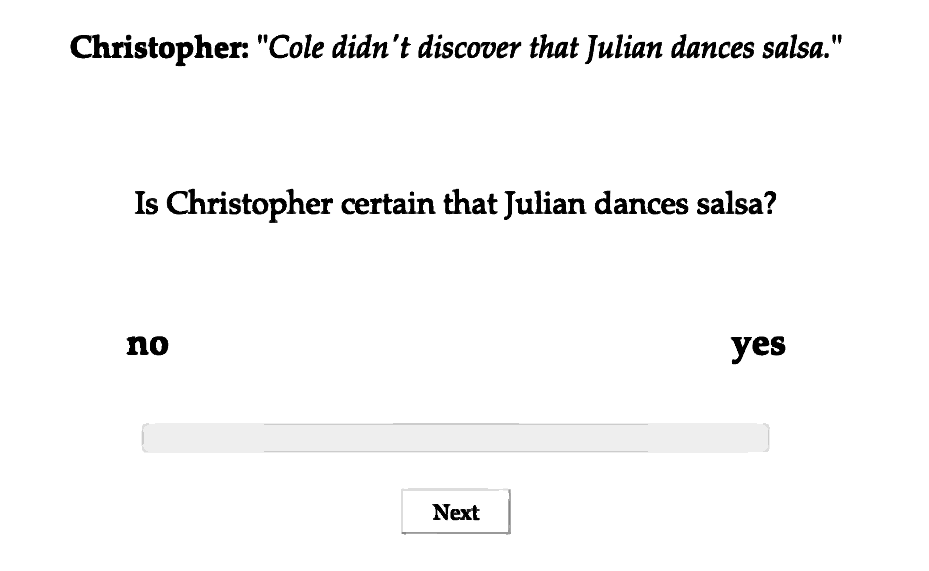
\includegraphics[width = .7\linewidth]{task-1n-proj.eps}
				\caption{A sample trial in Exp.~1. In the corresponding trials in Exps.~2-4, participants were presented with an utterance involving a different entailment-cancelling operator.}
				\label{fig:trial}
			\end{figure}
		

	\subsection{Results and discussion}
		Our analysis reveals two key results: \textbf{(i)} There is projection variability by operator and \textbf{(ii)} there is by-predicate variation in the effect of operator on projection.

		\subsubsection{By-operator variation}

			We find an effect of operator when aggregating across predicates. Mean projection ratings were higher under question-embeddings than under negation and modals, but lower than in conditional antecedents. This is shown in Fig.~\ref{fig:op-ratings}, and the generalizations are supported by Model \#1 reported in Table~\ref{t:op-model}.

			\begin{figure}[ht]
				\centering
				\includegraphics[width = .35\linewidth]{projective-op}
				\caption{Mean certainty ratings by operator with $95\%$ bootstrapped confidence intervals.}
				\label{fig:op-ratings}
			\end{figure}

			\begin{table}[ht]
					\centering
					\hspace{-1.3em}
					\begin{tabular}{llrrrr}
						Model & & Estimate & Std. Error & t-value\\
						\midrule
						\#1 & Intercept: \emph{question} & 0.51 & 0.01 & 44.78 & ***\\
						& operator: conditional & 0.05 & 0.01 & 5.30 & ***\\
						& operator: modal & -0.04 & 0.01 & -4.45 & ***\\
						& operator: negation & -0.03 & 0.01 & -4.67 & ***\\
						\bottomrule
					\end{tabular}
				
					\caption{Excerpt from the model output of a linear mixed effects model with fixed effects of operator; random effects: participant and item intercepts, fit with \texttt{lme4, lmertest} in \texttt{R}.\label{t:op-model}}
				\end{table}

			This result differs from that of \cite{sieker_projective_2022}, who observed that the CC of German attitude predicates projects more from under negation than the other operators.

			\begin{itemize}
				\item but like them, we observe small differences 
				\item overall, they have much higher projection ratings
				\item but they chose a different set of predicates, we can understand these different results when taking into account by-predicate variation in the effect of operator
			\end{itemize}

		\subsubsection{By-predicate variation in the effect of operator}

			We observe differences across the predicates in by-operator variation. This is illustrated in Figure~\ref{fig:op-pred-ratings}, which shows mean projection ratings for the 20 attitude predicates by embedding operator; predicates are ordered by their mean rating across all operators (\emph{be annoyed} has the highest overall mean).
			%
			For instance, whereas the CC of \emph{be annoyed} projects more from under negation and questions than conditionals and modals, and the CC of \emph{discover} projects less from negation than conditionals and questions, and more from under negation than modals. The CC of \emph{know} projects less from under negation than questions, but more from under negation than modals, while the difference between negation and conditionals is not significant.
			%
			These generalizations are supported by models\ \# 2--4 in Table\ \ref{t:models}, which also each have at least $34$ highly significant interaction terms (out of $57$ possible interactions of operator and predicate).

			\begin{figure}[ht]
				\centering
				\includegraphics[width = \linewidth]{projective-pred-op}
				\caption{Mean certainty ratings by predicate and operator with 95\% bootstrapped confidence intervals. Embedding operator coded by letter and color:  \texttt{N} (light blue): negation, \texttt{M} (orange): modals, \texttt{C} (green): conditional antecedents, \texttt{Q} (dark blue): polar questions.}
				\label{fig:op-pred-ratings}
			\end{figure}

			\begin{table}[ht]
				\centering
				\begin{tabular}{llrrrr}
					Model & & Estimate & Std. Error & t-value\\
					\midrule
					\#2 & Intercept: \emph{\bf be annoyed}/negation & 0.87 & 0.01 & 79.86 & ***\\
					& operator: conditional & -0.12 & 0.02  & -7.36 & ***\\
					& operator: modal & -0.16 & 0.02  & -10.01 & ***\\
					& operator: question & 0.02 & 0.01 & 1.72 & n.s.\\
					\midrule
					\#3 & Intercept: \emph{\bf discover}/negation & 0.68 & 0.01 & 62.70 & ***\\
					& operator: conditional & 0.11 & 0.02 & 7.11 & ***\\
					& operator: modal & -0.06 & 0.02 & -3.63 & ***\\
					& operator: question & 0.10 & 0.01 & 7.08 & ***\\
					\midrule
					\#4 & Intercept: \emph{\bf know}/negation & 0.79 & 0.01 & 72.97 & ***\\
					& operator: conditional & 0.00 & 0.02 & -0.06 & n.s.\\
					& operator: modal & -0.14 & 0.02 & -9.18 & ***\\
					& operator: question & 0.08 & 0.01 & 5.67 & ***\\
					\bottomrule
				\end{tabular}
				\caption{\small Excerpt of the output from three linear mixed effects models, with fixed effects: operator, predicate, and their interaction; random effect: participant intercepts.
				Models were fit with \texttt{lme4, lmertest} in \texttt{R}. Models \textbf{\#2--4} also had at least $34$ highly significant interaction terms of \texttt{operator} and \texttt{predicate} with $p < 0.001$ (not shown here).\label{t:models}}
			\end{table}

			This result that by-operator projection variability interacts with predicate concurs with \citet{smith_relationship_2014}, while we did not reproduce their result that the CC of \emph{know} projects more from negation than conditionals. This differs from the result of \citet{sieker_projective_2022}, who found no interaction between predicates and operators.
			%
			Given that the methods and the set of projective contents of our experiment were very similar to theirs, this difference may suggest cross-linguistic variation in projection variability (cf. \citealt{tonhauser_projection_2020}).

		\subsubsection{Gradience and lexical classes}

			Finally, our results provide further support (from negation, modals, and conditionals) for the result of \citet{degen_are_2022}, that projection does not categorically differentiate between (semi-)factive and non-factive predicates, while also replicating it for polar questions. 
			E.g., the CCs of non-factive \emph{inform} and \emph{acknowledge}, for instance, are at least as projective as that of some (semi-)factive predicates.

			Similarly, our results question \posscite{karttunen_observations_1971} proposed difference between factive and semi-factive predicates, in line with \citet{sieker_projective_2022} (see also \citealt{beaver_have_2010}): Although our data replicate the result from \citet{tonhauser_how_2018} that, in polar questions, the CC of semi-factive \emph{discover} is less projective than that of \emph{know}, the same does not hold in conditionals.
			%
			Further, contrary to what would be expected based on \posscite{karttunen_observations_1971} distinction between factive and semi-factive predicates, the CC of (factive) \emph{be annoyed} does not project invariably from all four operators, and the CC of \emph{discover,}  which is considered semi-factive, does not project more from under negation than the other three operators. The pattern observed for {\em know} does not fit into either category.

		\subsubsection{Converging evidence for operator / predicate interactions}
			MegaVeridicality dataset (\citealt{white_role_2018}): 517 predicates in three sentence types

			\ex. \a. Somebody didn’t know that a particular thing happened. (Did that thing happen?)
				\b. If somebody knows that a particular thing happened, did that thing happen?
				\b. If somebody didn’t know that a particular thing happened, did that thing happen?
				\z.
			\z.


			\begin{figure}[ht]
				\centering
				\includegraphics[width = \linewidth]{mega-veridicality}
				\caption{Mean projection ratings by embedding context and predicate.}
				\label{fig:figure1}
			\end{figure}

	
		\subsubsection{Interim conclusion}

			Results:

			\begin{enumerate}
				\item Effect of operator on projection

				\item Effect of operator on projection differs by predicate

				\item By-predicate variation on operator effects are gradient and cannot be predicted by categorical lexical classes

			\end{enumerate}

			Methodological implications:
			\begin{itemize}
				\item projection ratings do not categorically distinguish between lexical classes (e.g., factives, semi-factives, veridical predicates), so future research appealing to these categories must clarify their definition.

				\item Additionally, claims about projection variability must be relativized to the entailment-canceling operator.

				\item but we can still use FoS test in teaching, JT made this claim, but I don't understand the argument... help?

			\end{itemize}

			Theoretical implications: Accounts of projective content need to take into account predicate/operator interactions, and the gradient by-predicate variability. The following section argues that our results provide evidence for a triggering algorithm based on contextual rather than lexical or conceptual information (e.g., in the sense of \citealt{abrusan_predicting_2011,simons_best_2017}), and that the input to this triggering algorithm should be contextual rather than lexical inferences (e.g., in the sense of \citealt{schlenker_triggering_2021}).


\section{Theoretical implications}
	Our results---that projection is modulated by entailment-canceling operators, that there is by-predicate variation in the effect of operator on projection, and that this variation is gradient in ways that cannot be predicted by categorical lexical classes---are not captured by contemporary projection analyses, for several reasons.

	Here, we discuss (i) dynamic approaches, which assume that projection is determined lexically for factive predicates (\citealt{heim_projection_1983,heim_presupposition_1992,van_der_sandt_presupposition_1992}), (ii) approaches which assume that projection is determined by a contextual triggering algorithm that operates over the lexical entailments of an utterance (\citealt{abrusan_predicting_2011,simons_best_2017}), and (iii) approaches with a conceptual triggering algorithm that operates over contextual entailments of an utterance (\citealt{schlenker_triggering_2021}). While all of these approaches meet limitations in accounting for our data, we argue that the observed gradient effects of predicate/operator interactions favor integrating insights from competing accounts, namely a contextual triggering algorithm (as in \citealt{abrusan_predicting_2011,simons_best_2017}) operating over contextual set of inferences (as in \citealt{schlenker_triggering_2021}).

	- effect of different entailment-cancelling operators, not captured (heim vs santd, if projects projects; abtrusan operators?; schlenker can be imagined) in all systems it is conceivable, but no systemaitc itneraction spelled out


	- rely on lexical classes, factives, veriudical, no predictions of non-veridicals

	- not capture how the operator differentially affects different predicates (contextual entailment may provied an approach, but also needs to be spelled out yet)

	The first is that contemporary analyses do not lead us to expect interactions with different types of entailment-cancelling operators. While it is conceivable for the meaning of the operator to systematically interact with the possibility of local accommodation, no such interaction has been spelled out systematically.

	
	The second reason is that many contemporary analyses do not make predictions for the projection of the CC of many of the 20 predicates, as they are limited to (semi-)factive predicates, whose CCs are analyzed as presuppositions (e.g., \citealt{heim_projection_1983,van_der_sandt_presupposition_1992}), or entailed CCs that project unless at-issue with respect to the Question Under Discussion (e.g., \citealt{abrusan_predicting_2011,simons_best_2017}). A possible exception is the analysis of \citealt{schlenker_triggering_2021}, which predicts the potential for projection for CCs that are contextually entailed. In a full talk, we would like to discuss how this analysis might be extended to capture the gradient projection observed in our experiment.
	
	The third reason is that contemporary projection analyses do not make sufficiently fine-grained distinctions between different clause-embedding predicates (but only between whether the CC is a presupposition or entailed). Consequently, they do not make predictions about the by-predicate variation in the effect of operator on projection.


	\subsection{Factivity: Lexical triggering}

		In \citet{heim_projection_1983}, for instance, the CC of (semi-)factive predicates projects to the global context, except when that would produce an inconsistency, in which case the CC is accommodated to the local context of the operator.

	\subsection{Entailments and contextual triggering}

	\subsection{Contextual entailment and conceptual triggering}

	\subsection{Conclusion: Contextual entailment and contextual triggering}
		\begin{itemize}
			\item contextual entailments (but weaker notion of entailment)

			\begin{itemize}

				\item cant believe its not lexical roberts

				\item pragmatics of full embedding context; Does Cole think that Julian dances salsa? 

				\item why would that be the case?

			\end{itemize}

			\item contextual triggering

			\begin{itemize}

				\item what is the difference between know and prove (in terms of conceptual precondition, causal model?) there is no conceptually inherent relation between the two, the difference is lexical

				\item QUD influences

				\item what is the relationship between lexical differences and QUD?

			\end{itemize}

		\end{itemize}




\section{Lexical differences}

	In spite of a lack of categorical distinctions about the projection behavior of our verbs, we can find some interesting initial generalizations over lexical properties, indicated in \textbf{Figure\ 2}.

	So, can the observed interaction between predicate and operator in mean projection ratings be predicted from lexical semantic/pragmatic properties of the predicates, and, if so, how?
	This is a pressing question for future research, to which our data offer some tentative answers. We identify four major patterns.
	%
	The predicates \emph{pretend} and \emph{think} exhibit the {\bf `Negation high'} pattern, shown in panel (a) of \textbf{Figure~2}: We tentatively hypothesize that negation (but not the other operators) interacts with the semantic or pragmatic antiveridicality associated with these predicates.
	%
	The inferential predicates \emph{prove, confirm}, and \emph{establish} exhibit a {\bf `Negation low'} pattern, shown in panel (b): Here, we tentatively hypothesize that the veridical meaning component interacts with negation (but not the other operators), to result in lower projection ratings under negation.
	%
	For \emph{announce, confess, admit}, and \emph{reveal}, the CC is most projective when embedded in conditional antecedents: This {\bf `Conditional high'} pattern (c) may suggest that the discourse effect of a conditional interacts with the change-of-state communication predicates.
	%
	Finally, the predicates  \emph{inform, know}, and \emph{be annoyed} exhibit a {\bf `Modal low'} pattern (d). The lexical meaning of these predicates, whose CCs are among the most projective, appears to interact with the modal adverb {\em perhaps}, yielding lower projection ratings.

	%%%%
	In spite of a lack of categorical distinctions about the projection behavior of our verbs, we can find some interesting patterns. \textbf{Fig.~\ref{fig:figure2}} gives the mean certainty ratings for the four operators by predicate, identifying some groups of predicates that show similar by-operator variation. We highlight four \lq projection-profiles\rq here: \emph{pretend} and \emph{think} are the only predicates that are most projective under negation compared to all other operators (\texttt{N} $>$ \texttt{M, Q, C}). \emph{annouce, confess, admit,} and \emph{reveal} are most projective under conditionals, while there is also a tendency that there is more projection from questions compared to modals and negation, a difference that may not be robust for \emph{announce} (\texttt{C} $>$ \texttt{Q} \textcolor{gray!40}{$>_?$} \texttt{M, N}). \emph{prove, confirm,} and \emph{establish} are more projective under modals and conditionals than under questions and negation (\texttt{M, C} $>$ \texttt{Q, N}). Finally, \emph{inform} and \emph{know} are most projective under questions, and least projective under modals (\texttt{Q} $>$ \texttt{N, Q} $>$ \texttt{M}).
	
\section{Conclusion}


\newpage
\bibliographystyle{sub-chicago}
\bibliography{projection}

\end{document}
